\section{Polovodičové paměti}
\label{sec:polpameti}
Paměť je médium, které umožňuje uchovávat informace.
Základní paměťová buňka uchovává jeden bit informace - buďto logickou 0 nebo logickou 1.
Osm takových buňek tvoří jeden bajt.
Paměťové prvky jsou spojeny řádkovými a sloupcovými vodiči, pomocí kterých je možné je elektronicky ovládat.\\ \\
Parametry pamětí: \\
\begin{tabularx}{\linewidth}{l|l|l}
  \textbf{Parametr}  & \textbf{Jednotka} & \textbf{Popis}                                                        \\
  \hline
  Kapacita           & Bajt              & Množství informací, které lze do paměti uložit                        \\
  \hline
  Přístupová doba    & Sekunda           & Doba, od zadání požadavku, než paměť zpřístupní požadovanou informaci \\
  \hline
  Přenosová rychlost & Bajt za skundu    & Množství dat, které lze přečíst/zapsat za sekundu                     \\
  \hline
  Šířka toku dat     & Bit               & Počet bitů, které se po sběrnici přenášejí současně                   \\
  \hline
  Cena za bit        & Koruna za bit     & Cena za jeden bit paměti.                                             \\
  \hline
  Spolehlibost       & Sekunda           & Střední doba mezi 2 poruchami                                         \\
\end{tabularx}
\subsection{Dělení pamětí}
\subsubsection{Podle určení}
\begin{description}
  \item[Registry] - Paměti na čipu procesoru pro krátkodobé uložení dat.
    Malá kapacita, ale velmi vysoká rychlost.
  \item[Vnitřní] - Paměti na základové desce, slouží jako paměť programů a jejich data.
  \item[Vnější] - Vyměnná média a disky.
    Data jsou zaznamenávána magneticky, elektricky nebo opticky.
\end{description}
\subsubsection{Podle principu činnosti}
\begin{description}
  \item[Statická] - Pamět uchovávají informaci po dobu přívodu el. napětí.
    Mají nízkou přístupovou rychlost, ale jsou složité a drahé (Cache).
  \item[Dynamická] - Ztrácí informaci i když jsou připojené k el. napětí, proto je nutné je periodicky oživovat.
    Tvoří je transistor a kondenzátor. Mají vyšší přístupovou dobu, ale nižší náklady (Operační paměť).
\end{description}
\begin{multicols}{2}\centering
  SRAM
  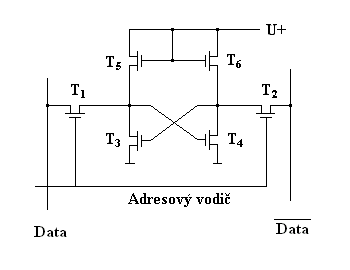
\includegraphics[width=\linewidth]{TVY-POS/Polovodicove-pameti/SRAM.png}
  \columnbreak\centering\\
  DRAM
  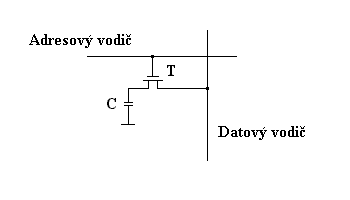
\includegraphics[width=\linewidth]{TVY-POS/Polovodicove-pameti/DRAM.png}
\end{multicols}
\subsubsection{Podle destruktivnosti při čtení}
\begin{description}
  \item[Destruktivní] - Paměť po přečtení informace ztrácí tuto informaci a je nutné ji znovu zapsat.
  \item[Nedestruktivní] - Uchovává informaci i po jejím přečtení.
\end{description}
\subsubsection{Podle energetické závilosti}
\begin{description}
  \item[Volatilní] - Paměť \textbf{NE}uchovává informaci po odpojení od el. napětí.
  \item[Non volatilní] - Paměť uchovává informaci i po odpojení od el. napětí.
\end{description}
\subsubsection{Podle přístupu}
\begin{description}
  \item[Sekvenční] - Před zpřístupněním informace je nutné přečíst všechny předcházející informace
  \item[Přímý] - Je možné přečíst přímo požadovanou informaci za pomocí její adresy
\end{description}
\subsubsection{Podle možnosti zápisu a čtení dat}
\begin{description}
  \item[ROM] - Data jsou zapsána při výrobě paměti. Realizováno vodičem nebo transistorem.
  \item[RWM] - Umožňují minimálně jeden zápis. Lze relizovat pomocí:
    \begin{description}
      \item[PROM] - Přepolování drátků. Pouze jeden zápis.
      \item[EPROM] - Elektronický zápis a mazání pomocí UV. Možnost více zápisů.
      \item[EEPROM] - Elektronický zápis i čtení. Možnost více zápisů.
    \end{description}
\end{description}
\subsubsection{Podle technolgie}
\begin{description}
  \item[Bipolární] - Buňky jsou tvořené bipolárními tranzistory
  \item[Unipolární] - Buňky josu tvoření tranzistory MOS
\end{description}
\subsection{R/W Cyklus buňky}
Vždy je udána adresa paměťového místa, se kterým se pracuje.
Adresa je přivedena na vstup dekoréru, která podle ní nastaví adresový vodič na log. 1.
Jestliže buňkou na tomto adresném vodiči projde log. 1 na datový vodič, tak je hodnota bitu log. 1. a vice versa.
U zápisu je dána opět adresa místa, kam se bude zapisovat, poté se nastaví hodnoty jednotlivých bitů a zapíšou se.
Způsob zápisu záleží na technologii buňky.
Buďto se buňka vypálí, nebo se otevře/zavře transistor, nabije/vybije kondenzátor.\\
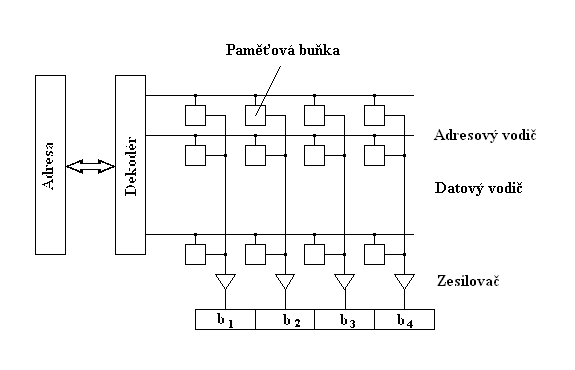
\includegraphics[width=\linewidth]{TVY-POS/Polovodicove-pameti/memorystructure.png}